\documentclass[dv_diss_main.tex]{subfiles}





%---------------------------------------------%
%----------------Figures----------------------
%---------------------------------------------%



\newcommand{\rddplot}{
\textit{Note.}This plot aggregate data into bins of half percentage points and estimate a third order polynomial regression between the running variable and the bins on each side of the cut-off. 
}


\newcommand{\rdd}{
\textit{Note.}This table reports the estimates of political alignment from equation (2). The sample includes post electoral years of all municipalities with close elections during the period 1998-2003. The outcome variables are measure as a three year changes. Controls refers to state fixed effects, election-year fixed effects, and baseline political characteristics (incumbency status, previous political alignment, previous political party). Mean dep var refers to the sample average of the outcome variable for the non-aligned municipalities. 
}



\newcommand{\sharerev}{
Percentage of revenues is the sample average share of each source of revenue on total revenues for the non-aligned counterparts
}

\newcommand{\shareemp}{
Percentage of employment is the sample average share of each sector on total employment for the non-aligned counterparts
}

\newcommand{\event}{
\textit{Note.}The figure plots the coefficients obtained from the estimation of equation (3) discussed in Section 4. The sample includes all municipalities with close elections during the period 1998-2003. The unit of observation is  the municipal-election pair, for each pair I follow the outcome measures in [-4 +4] years window. The outcome variables are measure in inverse hyperbolic sine points. The tick(thin) lines are 90\%(95\%) confidence intervals. The specification controls by municipality-election and election-year fixed effects. 
}

%inverse hyperbolic sine (IHS) transformation


\newcommand{\stars}{
Standard errors clustered at municipality level.  *** p<0.01, ** p<0.05, * p<0.1.
}

\newcommand{\census}{
}

\newcommand{\household}{
}

%example \newcommand{\rddnote}{\figtext{\justifying{\scriptsize{Notes:                }}}}
\newcommand{\starnotes}{* denotes significance at 10 pct., ** at 5 pct., and *** at 1 pct. level.}


%---------------------------------------------%
%----------------Figures----------------------
%---------------------------------------------%

%---External validity 

\newcommand{\sammi}{
\textit{Note.}This figure presents the difference of means of baseline covariates from the 2000 population census. Each point represents the estimate of the difference in means and the line the corresponding 95 percent confidence interval. All variables are standardized. Panel A shows the difference in means between the observational sample and the OLS-weighted sample. Panel B shows the difference in means between the observational sample and the IV-weighted sample. IV model weights are estimated using a control function approach. The weights are computed  based on Aronow and Samii (2016). We include as controls time and municipality fixed effects, formula's inputs and pre-trends of all outcomes of interest.
}

\newcommand{\sammidescrip}{
	
\textit{Note.}Means and standard deviations for baseline covariates from the 2000 population census. The column of the observational sample refers to the unweighted average. The OLS and IV columns correspond to weighted averages using regression-based weights of the corresponding models. The weights of the IV model are estimated using a control function approach. The weights are computed  based on Aronow and Samii (2016). We include as controls time and municipality fixed effect, formula's inputs and pre-trends of all outcomes of interest.

}

\newcommand{\revenuebydecil}{
\textit{Note.} Calculations based on information from SIMBAD (State and Municipal System Databases), National Institute of Statistics and Geography (INEGI).
}


\newcommand{\povertylineformula}{
\textit{Note.} The Figure shows the poverty line used to compute the formula on a yearly basis. We did not include the 2001 poverty line (Mex\$1097.859) for visualization purposes. Our estimation sample includes FAIS resources allocated between 2002-2014. 

}


\newcommand{\faisvariation}{\textit{Note.} The Figure plots the distribution of the share of transfer that corresponds to each state according to the FAIS formula. The figure plots the distribution of the demeaned shares across years by state  (2002-2014). Source: State FAIS formula values are collected from the Official Federal Gazette publication made on October of every year. }
\newcommand{\pcinequality}{
\textit{Note.} Calculations using the poverty maps of 2000, 2005, 2010, and 2014. Each quantile group is approximately 112 municipalities.
}

\newcommand{\pcincomegrowth}{
\textit{Note.} numbers reported are average across municipalities. The index shows the changes in a given percentile of the  municipal household income per capita distribution. Municipalities at the nth percentile in 2000 and 2014 do not necessarily correspond.
Source: Calculations using the poverty maps of 2000, 2005, 2010, and 2014.
}

\newcommand{\figurefaistrends}{
	
\textit{Note.}Panel A plots the share of municipalities reporting to receive zero resources from FAIS. Panel B plots the average value of per-capita transfers in constant prices, normalized to be 1 in 2005. Other public revenues include taxes, debt and unconditional cash transfers

}




%---------------------------------------------%
%----------------Tables----------------------
%---------------------------------------------%

\newcommand{\maintable}{\textit{Note.}Table entries correspond to separate regressions of an outcome,  listed on the leftmost column, on the independent variable specified in the column titles. Observations are the same across specifications that are in the same column. All monetary variables (intergovernmental transfers  and household per-capita income percentiles) are in logs, coverage and poverty headcount variables are in percentage points. Standard errors (in parentheses) are clustered at the municipality level to reflect the design effect and the autocorrelation of shocks over time. 2SLS estimates report the Kleibergen-Paap rk Wald F-statistic [in brackets]. 
}


\newcommand{\indicestables}{\textit{Note.}Table entries correspond to separate regressions of an outcome,  listed on the leftmost column, on the independent variable specified in the column titles. Observations are the same across specifications that are in the same column. All the outcomes indices that aggregate the information of all the variables that belong to a specific family. The infrastructure index aggregates the information of access to electricity, connection to sewerage, access to water,
quality of floor and access to sanitation. The poverty index aggregates the information of the inverse of log of per capita income and poverty rates measured by three poverty lines (food, capabilities and assets). The inequality index aggregates the information of Gini index and all income rations considered in the main results (90/10, 50/10 and 90/50). The index of each family is a linear combination of all the variables that belong to each family where the weights are based on \cite{anderson2008multiple}. Standard errors (in parentheses) are clustered at the municipality level. All  2SLS estimates report the Kleibergen-Paap rk Wald F-statistic [in brackets].
}


\newcommand{\firststage}{
\textit{Note.} The horizontal axis scale in logs but axis labels measure in constant pesos per capita of 2014. The plotted values correspond to mean-standardized residuals from transfers on a set of controls. Each color corresponds to a different specification: i) Purple, labeled as FE, includes municipality and time fixed effects. ii) light blue, labeled as FE+ Controls, includes the same set of fixed effects and two sets of time-varying controls: a) formula inputs, b) pre-policy trends outcome trends for all our outcomes of interest. 
}


\newcommand{\firststagetable}{
	\textit{Note.} This table presents estimates from regressing observed FAIS on law-implied FAIS transfers. Standard errors (in parenthesis) are clustered at the municipality level. Panel A adds sequentially the controls of our baseline specification across columns. The other panels add on top of that other set of time-varying controls. Panel B adds over the specifications of panel A the following sociodemographic controls: proportion of the adult population by education levels (primary, secondary and tertiary), the proportion of males and the dependency ratio. Panel C adds over the specifications of panel A the following economic controls: proportion of workers by sector (agriculture, manufacturing, construction, commerce, low-skill services and high skill services) and proportion of workers by type of occupation (abstract non-routine task, routine task, manual task, and non-routine manual tasks). 
	%Panel D adds over the specifications of panel A the following political controls: the size of public sector, the share of public workers with tertiary education, local revenue sources by type(own revenue, intergovernmental transfers both earmarked and non-earmarked). 
	In column (3) we use the assets poverty rate as a reference outcome to define the control used for pre-trends; results are robust to using any other outcome of interest as reference. \\
	\starnotes
}


\newcommand{\trendsdescrip}{
	\textit{Note.} Table entries in columns (1) and (2) correspond to separate regressions of an outcome, listed on the leftmost column, and our instrument in column titles. Outcome variables were measured as annual change between 1990 and 2000s. Coefficient estimates and robust standard errors (in parenthesis) correspond to cross-sectional regressions. Column (1) shows the unconditional correlation between the pre-policy trends and our instrument. Column (2) adds the formula's inputs as controls. Column (3) shows the mean and standard deviation of the pre-policy trends, measure as the average annual difference between 2000's and 1990 values. \\
	\starnotes
}




\newcommand{\mainresults}{
Column (1) reports OLS estimates of observed FAIS on outcomes of interest.
Column (2) reports reduce form estimates of law-implied FAIS.
Column (3) to (5) reports instrumental variable estimates of observed FAIS instrumented by law-implied FAIS. Column (3) includes standard controls, Column (4) has as additional control trends of the outcome of interest for the pre-policy period (1990-2000) interacted with year dummies. Column (5) includes time varying measures of all other source of municipal revenues: taxes, unconditional transfers and other conditional transfers. \\
\starnotes
}

\newcommand{\polynomial}{
	Column (1) reports our baseline specification for comparison purposes.
	Column (2) and Column (3) reports estimates from a specification that include as controls second and third order polynomials of the formula inputs. \\
	\starnotes
	
}

\newcommand{\trend}{
	Column (1) reports our baseline specification not accounting by pre-trends. 
	Column (2) corresponds to our baseline specification, it controls by pre-trend using the annual change in the outcome of interest between 1990-2000 interacted with a year dummy.
	Column (3) controls by pre-trends using the predicted level of the outcome of interest under linear trends assumption. 
	Column (4) controls by pre-trends using the lagged value of the outcome of interest. \\
	\starnotes
}

\newcommand{\urban}{
	Column (1) reports our baseline specification applied to the entire sample. 
	Column (2) reports our baseline specification for the subsample of municipalities with more than 15,000 inhabitants. Column (3) reports our baseline specification for the subsample of municipalities with less than 15,000 inhabitants. \\
	\starnotes
}





\newcommand{\mhtnote}{
		\textit{Note.} Table entries correspond to separate regressions of an outcome, listed on the leftmost column, on the variable specified in the column title. This table  present the estimates of our preferred specification, which corresponds to estimates of column 4 in Tables~\ref{tab:3},~\ref{tab:4} and~\ref{tab:5}. Standard errors (in parentheses) are clustered at the municipality level to reflect the design effect and the autocorrelation of shocks over time. Sharpened false discovery rate (FDR) q-values following Anderson (2008) in [brackets]. Family-wise p-values based on 2,000 bootstraps of the free step-down procedure of Westfall and Young (1993) in \{curly brackets\}. All monetary variables (intergovernmental transfers and household per-capita income percentiles) are in logs, coverage and poverty headcount variables are in percentage points. 
		\\
		\starnotes using conventional inference. 
}


\newcommand{\spendingcatalog}{
\textit{Note.}Each pair of Classification and sub-classification defines an authorized line  of spending authorized by FAIS spending catalog. Type abbreviations: Direct (D), Indirect (I), Complements (C.) and Specials (S)-most commonly used for natural disasters emergencies-. Modality abbreviations: C means construction, Eq means equipment, Ex means extension, I means installation, M means maintenance, R means rehabilitation, S means substitution, pre means preschool, pri means primary school, sec means secondary school and prep means high school. Source: Lineamientos Generales para la operación del FAIS (Anexo 1), February 14, 2014 https://ww.dof.gob.mx/nota_detalle.php?codigo=5332721&fecha=14/02/2014.
}


% Regressions include but do not report the lagged dependent variable, fixed effects for randomization blocks, and a set of LASSO-selected baseline covariates, and are weighted be representative of the eligible population. Standard errors (in parentheses) are clustered at the household level to reflect the design effect. Asterices denote significance at the 10, 5, and 1 percent levels, and are based on clustered standard errors, in parentheses. Anderson (2008) sharpened q-values presented in brackets. Variables marked with a † are in inverse hyperbolic sines. Reported p-values in final two columns derived from F-tests of hypotheses that cost-benefit ratios are equal between GD Main and Large transfer amounts (GD=GDL), and between Gikuriro and GD Large (GK=GDL).




\begin{document}


%\addcontentsline{toc}{subsection}{Online Appendix}
%\renewcommand{\thesubsubsubsection}{\Alph{subsubsubsection}}
%\counterwithin{figure}{subsubsubsection}
%\counterwithin{table}{subsubsubsection}

\normalsize
%\lmr
\normalfont



\subsection{Fondo de Aportaciones para la Infraestructura Social - FAIS}

\subsubsubsection{FAIS spending rules}\label{ap:faisspending}

Local governments can use FAIS resources in a wide array of public investment projects. These projects are listed in the operational guideline of the FAIS. The list covers more than 200 different projects under several modalities that are classified in 7 categories: education, health, housing, social assistance, urbanization, water and sanitation and others. 

The following table groups the potential projects by category, modality and associated social deprivation from the FAIS' service Catalog. For some spending categories marked with * (medical stall, equipment and medicine supply), the fund can be invested  if resources for the operation of the dental or health centers are provided by the federal government. Municipalities must spend at least 40 percent of the fund in direct projects (listed in Panel A) while the rest can be invested under their discretion.


\begin{table}[H]
	\centering
	\small
	\caption{FAIS Spending Rules Catalog}\label{fig:discon}
	\label{trends_inf}
	\resizebox{\textwidth}{!}{
		

\begin{tabular}{llcl}
		
		\toprule
		\textit{\textbf{Classification}} &\textit{\textbf{Subclassification}} & \textit{\textbf{Modality}} &  \textit{\textbf{Social Deprivation}}
		\\
		
		
		%%%%%
		\midrule
		\multicolumn{4}{l}{\textbf{Panel A. Type of Spending: Direct (D)}} 
		\\
		\vspace{0.2 cm} \\
		
		Education & School meals (pre, pri, sec) & C/Ex/M/Eq & Access to food
		\\
		 & Classrooms, Restrooms (pre, pri, sec, prep) & C/Ex/M/Eq& Educational gap
		\\
		\midrule
		\vspace{0.2cm}
		Health & Dental clinic* & C/Ex/M/Eq & Access to health
		\\
		 & Health clinic* & C/Ex/M/Eq & Access to health services
		\\
		\midrule
		\vspace{0.1cm}
		Housing & Rooms/Bathrooms/Kitchen & C & Quality and space of the dwelling
		\\
		 & Quality materials of the dwelling (walls, cement floor, roof) & C & Quality and space of the dwelling 
		\\ 
		 & Connection to drainage & C & Quality and space of the dwelling
		\\ 
		 & Ecological cookstoves & Eq & Quality and space of the dwelling
		\\ 
		\midrule
		Social Assistance & Community kitchens& C/Ex/M/R & Access to food
		\\ 
		
		Urbanization & Connection to electricity & C/I/Ex/M/S  & Basic services
		\\ 
		\midrule
		Water and Sanitation & Connection to water supply & C & Basic services
		\\
		 & Sump pump & M/R/Eq & Quality and space of the dwelling
		\\
		 & Drinking water (tank, wells, network, cistern) & C/M/S/R/Eq & Basic services
		\\
		 & Water treatment plant & C/M/S/R/Eq & Basic services \\ 
		 & Storm drain/sewer & C/Ex/M/R & Basic services 
		\\
		& Noria & C/M/R/Eq & Basic services 
		\\ 
		 & Artesian aquifer & C/M/R/Eq & Basic services
		\\ 
		 & Absorbing well & C/Ex/M & Quality and space of the dwelling
		\\ 
		 & Septic tanks connected to sewage & C/Ex/M & Quality and space of the dwelling
		\\ 
		%%%%%
		 \midrule
		\multicolumn{4}{l}{\textbf{Panel B. Type of Spending: Indirect (I)}} 
		 \\
		\vspace{0.2 cm} \\
		
		Education & Basic services (pre, pri, sec, prep) & C/Ex/M/Eq & Educational gap
		\\ 
		Water and Sanitation & Sewerage system & R/C/Ex/M & Basic services
		 \\
		 
		\midrule
		\multicolumn{4}{l}{\textbf{Panel C. Type of Spending: Complement (C)}}
		 \\
		\vspace{0.2 cm} \\
		Education & Fences (pre, pri, sec, prep) & C/Ex/M &
		\\ 
		Social Assistance & Shelters & C/Ex/Eq & 
		\\
		\midrule
		Others & Agricultural infrastructure & C/Ex/M/R & 
		\\ 
		 & Infrastructure for handcrafts & C/Ex/M/R &
		\\ 
		\midrule
		Urbanization& Roads, Streets, Highways & C/Ex/M/R &
		\\ 
		 & Sidewalks, Fords, Retaining walls, Signage & C/Ex/M/R & 
		\\ 
		 & Street lighting & C/Ex/M & 
		\\ 
		 & Infrastructure for the access of people with disabilities & C/Ex/M/R &
		\\ 
		\hline
		
		\bottomrule
	\end{tabular}
	
				}		
\parbox{\textwidth}{\small 
\vspace{2eX}
\footnotesize	
 \spendingcatalog
  
}
\end{table}

\subsubsubsection{FAIS Allocation Formula} \label{ap:faisformula}

This annex describes the details about the formula presented in the Article 34 added to the Fiscal coordination law in December 29 of 1997. The formula computes for every household a deprivation mass index that is based on the nonlinear combination of 5 dimensions indexed by $g=\{1,2,3,4,5\}$. The formula will be computed every year $t$ using the latest available population census indexed by $k$. This implies a one to one mapping between $t$ and $k$ defined by $k(t)$. Although in our identification strategy we use this notation, for simplicity we will drop any time subscript that index the round of population census used for the computations.


The formula that describes the deprivation mass at household level from the latest population census is as follows

$$D_{j} = \sum_{g} \omega^{g} f_{g} (W_{j}^{g}) $$



Where $D_{j}}$ is the deprivation mass of household $j$ in the population census. $\omega^g$ is the policy weight for characteristic $g$ and $W_{j}^{g}$ is a vector of household characteristics used to compute the dimension $g$ for household $j$. A specific function $f_{g}(.)$ is applied to $W_{j}^{g}$. Below we describe for each dimension the weights--$\omega_{g}$, functions--$f_{g}(.)$, and variables--$W_{j}^{g}$ employed to compute the household deprivation mass for each dimension
\\	
\\
{\bf Household per-capita income}-- This dimension has a weight of $\omega^{1}=0.46$. It use as characteristic the household per-capita income as input and compute a poverty gap measure. To do so, it requires an extreme poverty line defined every year $t$ by the Secretary of Development $l^_{t}$. This line is expressed in real values of the year of the latest population census available $k(t)$. We apply the formula as follows:

$$\frac{l_{t} - W_{j}^{1}}{l_{t}}$$

Where $W_{j}^{1}$ correspond to household per-capita income. Then we apply the following stepwise function to the poverty gap

$$
f_{1}(W_{j}^{1})= \left\{ \begin{array}{ccc}
	-0.5 &   if & $$\frac{l_{t} - W_{j}^{1}}{l_{t}}$$ <- 9 \\
	\\ $$\frac{l_{t} - W_{j}^{1}}{l_{t}}$$ \times \frac{1}{18} &  if & -9 <$$\frac{l_{t} - W_{j}^{1}}{l_{t}}$$<0 \\
	\\ $$\frac{l_{t} - W_{j}^{1}}{l_{t}}$$ &  if  & $$\frac{l_{t} - W_{j}^{1}}{l_{t}}$$ \geq 0
	%\left\{
\end{array}
$$
\\
\\
{\bf Household education level}-- This dimension has a weight of $\omega^{2}=0.125$. It is built with the relation between the education of each household member $ij$ with respect to its age as follows 

$$E_{ij} =  \frac{yrs\; of\; education_{ij}}{Norm\;(\;age_{ij}) } \times 1(literacy_{ij})$$

where  $Norm(age_{ij})$ is the normative of the years of education an individual of a specific age should have. $E_{ij}$ is equal to zero for iliterate household members older than 15 years old. Once $1-E_{ij}$ is obtained for each individual $ij$, it is evaluated in their corresponding step function $f_2()$ defined below:

$$ f_2(E_{ij})= \left\{ \begin{array}{ccc}
(1-E_{ij}) \times \frac{1}{7.33} &   if & 1-E_{ij} < 0\\
\\ 	1-E_{ij} & if & 1-E_{ij} \geq 0
% \left\{
\end{array}$$

To aggregated at household level, we take the average of household members for who  $E_{ij}$ has been computed. When controlling for these characteristics in our main estimates, we will control for the average years of education of people higher than 15 years old and for proportion of illiterate people. 
\\
\\
{\bf Household crowding}-- This indicator has a weight of $\omega^{3} = 0.2386$. It measures whether the occupancy of a dwelling exceeds a benchmark capacity, defined as three people per bedroom. The dimension measure is defined as follows

$$W_{j}^{3} = \frac{3 B_{j}}{N_{j}}$$

where $B_{j}$ and $N_{j}$ is the number of bedrooms and household members in household $j$. This measure is normalized by the following step-wise function:

$$f_{3}(W_{j}^{3})= \left\{ 
\begin{array}{lcl}
    -\frac{0.5}{75}\times W_{j}^{3}  &   if  & 1-W_{j}^{3} < 0 \\
    \\ 	1- W_{j}^{3}                 &   if  & 1-W_{j}^{3} \geq 0
\end{array}$$
\\
{\bf Access to Sewerage}-- This indicator has a weight of $\omega^{4}=0.0608$. It creates a mapping between each type of sewerage connection $W^{4}_j$ into a score as follows: 

$$f_{4}(W_{j}^{4})= \left\{ 
\begin{array}{lcl}
    1-1.5    &   if  &  main\; network \\
    1-1      &   if  & septic\; tank \\
    1-0.5    &   if  & tubewell\; or \; borehole \\
    1-0.3    &   if  & surface\; water\; (river,\; dam,\;etc\; ) \\
    1-0      &   if  & not sewearage\; system 
\end{array}$$
\\
\\
\newpage
\noindent{\bf Electricity or gas to cook}-- This indicator has a weight of $\omega^{5}=0.114$. This indicator measures whether the household has either electricity or an adequate fuel to cook. The vector of characteristics that are used for this indicator is $W^{5}_j$. Each household is assigned an specific numeric value according to the following mapping: 


$$f_{5}(W_{j}^{5})= \left\{ 
\begin{array}{lcl}
    1-1      &   if  & access\; to\; electricity \\
    1-1      &   if  & cook\; with\; gas \\
    1-0.5    &   if  & cook\; with\; oil \\
    1-0.3    &   if  & cook\; with\; wood \\
    1-0      &   if  & cook\; with\; charcoal
\end{array}$$


To aggregate at municipality level, the formula compute a weighted aggregate of the deprivation mass of each household only for those households which are considered poor under the deprivation mass measured

$$D_{m} = \sum_{j\in m} D_j^2 \times \;members_{j} \times 1(D_j>0) $$

\subsubsubsection{Sources of Variation in FAIS Formula}\label{ap:overtime}

The change of the formula over time is due to three sources of variation: First, the total FAIS pot at national level; second, changes in the poverty line that affects the formula; third, changes in round of the population census used to compute the formula. 

\begin{figure}[H] 
		\centering
		
		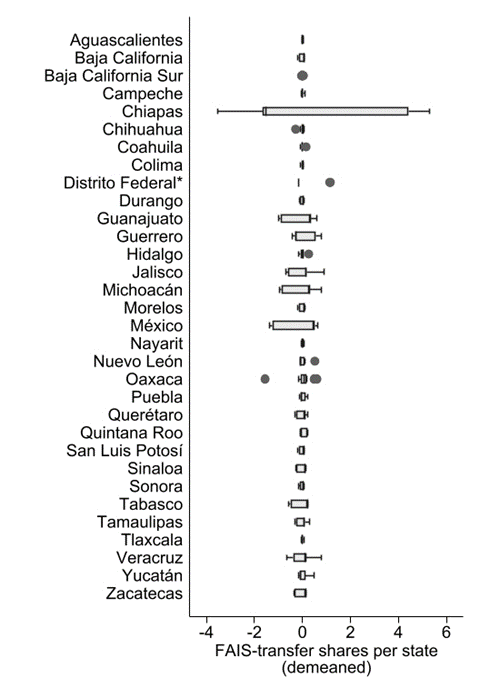
\includegraphics[width=0.67\linewidth]{figures/distribution_states.png}
		\caption{Deviation from Historical Share of FAIS Across States (2001-2015)}\label{fig:B1}
		
		\parbox{\textwidth}{\small 
		\vspace{2eX}
		\footnotesize	
		\faisvariation
		}
	
\end{figure}

The above shows the time variation at state level of the share of FAIS transfers. By plotting the shares we isolate over time variation that we obtain from changes in the FAIS' pot at national level. In case the census shock were the only important source of variation we should observe a bi-modal distribution, with two points, before and after the census shock. As it can be seen this is not the case, which means we also get identification from variation in the national poverty line that affects the formula.

Notice that our specification we control by formula's inputs, which means that the variation that we exploit from changing the population census used to compute the formula correspond to the non-linear implications of changing formula's inputs. 

Figure below shows the value of the poverty line updated every year by the Federal government. This update affects differently each municipality according to the height of the household income distribution around the poverty line.\footnote{ Remember the poverty defines the first dimension score, which has the largest weight in the deprivation mass at the household level.} 

\begin{figure}[H] 
	\centering 
	
		\centering
		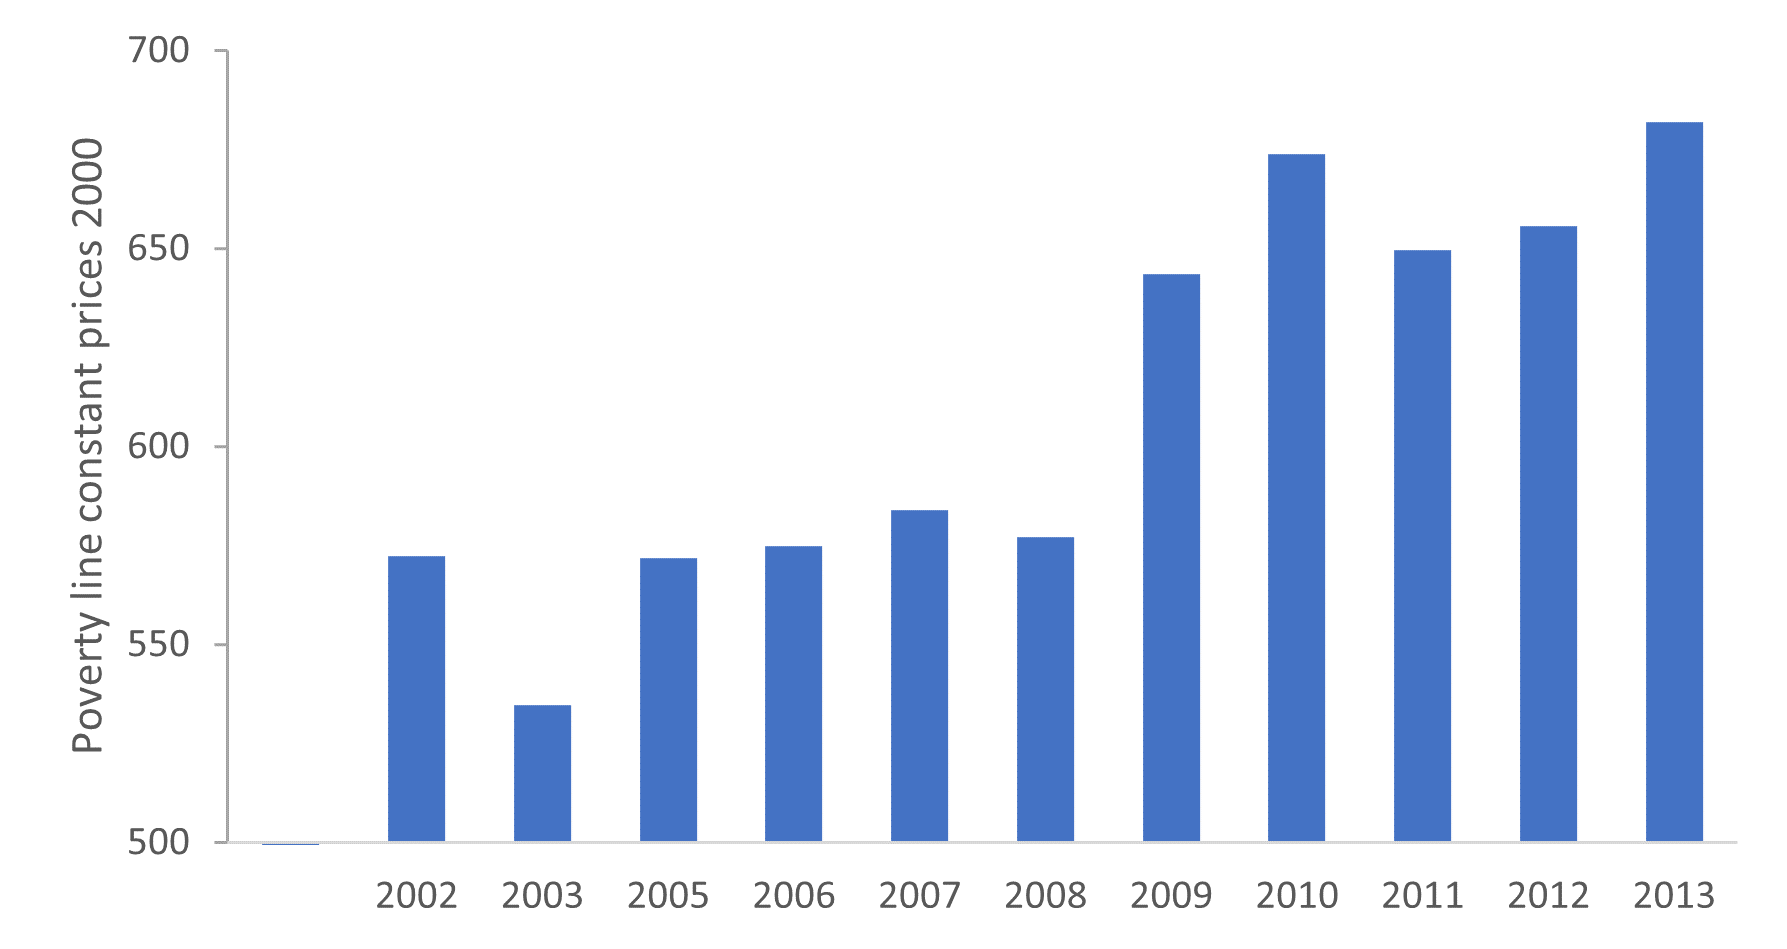
\includegraphics[width=\linewidth]{figures/Poverty_line.png}
		\vspace{0.1cm}
		\caption{Poverty Line Used to Allocate FAIS Transfers}\label{fig:B2}
		
		\parbox{\textwidth}{\small 
		\vspace{2eX}
		\footnotesize	
		\povertylineformula 
		}
	
\end{figure}

\subsection{Public Finance in Mexico}
    
\subsubsubsection{Revenues and Spending Categories in Public Finance Data} \label{Ap:fiscalcategories}

The National Institute of Statistics and Geography (INEGI) compiles all administrative records on the source and use of all financial resources in municipalities. This information is openly available through the State and Municipal System Databases (SIMBAD) on the INEGI website. The Figure below presents the maximum degree of disaggregation of public accounts at the municipal level available in SIMBAD. 
\begin{figure}[H] 
	\centering 
	
		\centering
		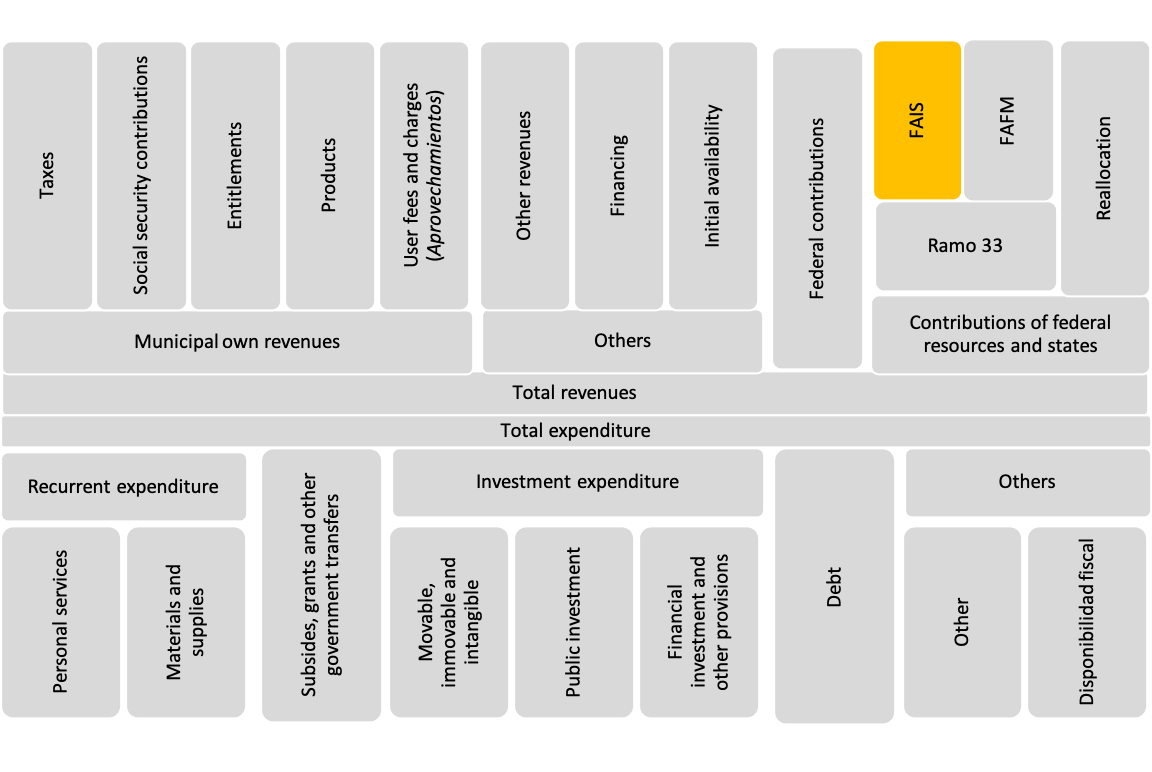
\includegraphics[width=0.8\linewidth]{figures/FAIS_in_local_finances.png}
		\caption{Fiscal Accounts, Municipal Level}\label{fig:discon}
	\vspace{0.1cm}
\parbox{\textwidth}{\small 
	\footnotesize	
	\textit{Note. }Constructed using SIMBAD (State and Municipal System Databases), National Institute of Statistics and Geography (INEGI).
	}
\end{figure}

\newpage

In our estimations we control for all other sources of fiscal revenues groped in the following categories:

\begin{itemize}
    \item Own revenues: Includes revenues from taxes, contributions to social security, products, and uses fees and charges
    \item Unconditional transfers: federal participation resources (known as Ramo 28)
    \item Conditional transfers: federal contribution (known as Ramo 33), here we include all transfer from Ramo 33 except those that correspond to FAIS.
    \item Other revenues: They usually come from resources not spent in previous years or other financial instruments
\end{itemize}


\subsubsubsection{Intergovernmental Transfers}\label{intertransfer}

Below a short description of how the main intergovernmental transfers work in Mexico. The idea is to provide evidence that the bulk of public spending allocated to municipalities does not follow similar rules than FAIS providing arguments for a exclusion restriction of our the FAIS formula.
\\
\\
{\bf Non-earmarked Transfers: Ramo 28 - Participaciones Federales}

\begin{itemize}
    \item 	Fondo General de Participaciones (FGP) - General Participation Fund. Allocation of resources to states, based on:
    \begin{itemize}
        \item Allocation received in 2007
        \item Economic growth
        \item Tax collection effort
        \item Size of the population
    \end{itemize}
    
    At least 20\% of the fund allocated to the state will be directly for the municipalities.
    
    \item Fondo de Fomento Municipal (FFM) - Municipal Development Fund. Allocation of resources is based on:

    \begin{itemize}
        \item Allocation received in 2013
        \item The surplus of each year with respect to 2013 is assigned:
        \begin{itemize}
            \item 70\% according to the growth in local collection of property taxes, water rights and the size of the population
            \item 30\% according to the growth in the collection of the property tax for municipalities where the state government of was responsible for the administration of the tax on behalf of the municipality
        \end{itemize}
        
    \end{itemize}
    
    \item Fondo de Fiscalización y Recaudación - Audit and Collection Fund Allocation of resources to states, based on:
    
   \begin{itemize}
   \item Allocation received in 2013
   \item The surplus of each year with respect to 2013 is allocated according to the evolution of:
        \begin{itemize}
            \item Audit indicators
            \item Tax collection growth in each state
        \end{itemize}
   At least 20\% of the fund allocated to the state will be directly for the municipalities.
   \end{itemize}
   
    \item 	Fondo de Extracción de Hidrocarburos (FEXHI) - Fuel Extraction Fund. The fund is distributed to oil-producing states according to:
    
   \begin{itemize}
   \item share of the total value of the gross extraction of fuel
   \item extraction value of associated gas and non-associated gas
        
   At least 20\% of the fund allocated to the state will be directly for the municipalities.
   \end{itemize}
   
\end{itemize}

{\bf Earmarked Transfers: Ramo 33 - Aportaciones Federales}
\begin{itemize}

\item 	Fortalecimiento de los Municipios (FORTAMUN) - Strengthening of Municipalities Fund
Allocation of resources to states, based on:
   \begin{itemize}
   \item 75\% is assigned according to the resident population
   \item 25\% based on the floating population 
        
   \end{itemize}

\item Earmarked Transfers: Conditional Cash Transfer - Prospera
   \begin{itemize}
   \item Selection of localities based on the marginalization index and social backwardness index (education, health, basic services and quality of the dwelling)
   \item Selection of eligible households within selected localities using proxy means test. The set of variables include: demographics, schooling, labor, access to social security, food access, access to health services, other income, characteristics of the dwelling, assets and social backwardness index at the municipal level. 
   
   Although it also focus on measures alike to FAIS index its computation is based on principal components with several different components than FAIS. Also since it use a PCA, it results form a linear o=combination of household characteristics.  

   \end{itemize}

\end{itemize}

\subsection{Pre-trends}\label{ap:c}

%Impact of FAIS on Social Infrastructure
%Impact of FAIS on Poverty and Mean Income
%Impact of FAIS on Inequality
%Impact of FAIS on the Income Distribution Percentiles


\begin{table}[H]
	\centering
	\small
	\caption{Pre-trends: Impact of FAIS on Social Infrastructure}
	\label{trends_inf}
	\resizebox{11cm}{!}{
		\begin{tabular}{lcccc}

\toprule



\multicolumn{1}{l}{} & \multicolumn{4}{c}{\footnotesize{Observed FAIS Transfers (2SLS)}} \\ 

\cmidrule(lr{1mm}){2-5}  % \\ was before, it was creating an extra additional line


\multicolumn{1}{l}{} &  \multicolumn{1}{c}{(1)} &
						\multicolumn{1}{c}{(2)} & 
						\multicolumn{1}{c}{(3)} & 
						\multicolumn{1}{c}{(4)}  \\ 


\midrule

%\multicolumn{7}{c}{\textit{Panel   A: Direct policy outcomes on infrastructure}} \\                                                          

% 1st row 
\textit{Access to electric lighting}   &  1.171***   &
						   0.912***   &
						   1.430***   &  
   						   1.342***   \\

\vspace{4pt} &  \footnotesize{(0.374)}  &
			    \footnotesize{(0.350)}  &
			    \footnotesize{(0.445)}  &
				\footnotesize{(0.437)}  \\

\vspace{4pt} &  \footnotesize{[844]} &
				\footnotesize{[830]} &
				\footnotesize{[600]} &
				\footnotesize{[602]} \\
				




% 2nd row 
\textit{Connection to sewerage}   &  6.219***   &
						   6.160***   &
						   7.625***   &  
   						   7.883***   \\

\vspace{4pt} &  \footnotesize{(0.978)}  &
			    \footnotesize{(0.975)}  &
			    \footnotesize{(1.181)}  &
				\footnotesize{(1.198)}  \\

\vspace{4pt} &  \footnotesize{[844]} &
				\footnotesize{[850]} &
				\footnotesize{[594]} &
				\footnotesize{[592]} \\
				


% 3rd row  			
\textit{Access piped water}   &  4.525***   &
						   4.945***   &
						   5.354***   &  
   						   5.485***   \\

\vspace{4pt} &  \footnotesize{(0.952)}  &
			    \footnotesize{(0.951)}  &
			    \footnotesize{(1.159)}  &
				\footnotesize{(1.148)}  \\

\vspace{4pt} &  \footnotesize{[844]} &
				\footnotesize{[855]} &
				\footnotesize{[596]} &
				\footnotesize{[593]} \\
				

% 4th row  				
\textit{Housing (floor quality)}   &  4.792***   &
						   4.175***   &
						   2.778***   &  
   						   2.814***   \\

\vspace{4pt} &  \footnotesize{(0.727)}  &
			    \footnotesize{(0.742)}  &
			    \footnotesize{(0.740)}  &
				\footnotesize{(0.755)}  \\

\vspace{4pt} &  \footnotesize{[844]} &
				\footnotesize{[761]} &
				\footnotesize{[579]} &
				\footnotesize{[577]} \\
				


% 5th row 
\textit{Access to sanitation}   &  -0.447   &
						   -0.288   &
						   -0.388   &  
   						   -0.495   \\

\vspace{4pt} &  \footnotesize{(0.550)}  &
			    \footnotesize{(0.586)}  &
			    \footnotesize{(0.598)}  &
				\footnotesize{(0.646)}  \\

\vspace{4pt} &  \footnotesize{[844]} &
				\footnotesize{[815]} &
				\footnotesize{[596]} &
				\footnotesize{[600]} \\
				


\midrule
{\bf Controls}    					&	   &   
										   & 
										   & 
										   \\


\textit{Municipality and year FE}    &	$\checkmark$   &   
										$\checkmark$   & 
										$\checkmark$   & 
										$\checkmark$   \\

\textit{Formula inputs}  	& 	$\checkmark$    &   
								$\checkmark$    & 
								$\checkmark$    & 
								$\checkmark$    \\


{\bf Pre-trends Control}       &	   &   
									   & 
									   &
									   \\

\textit{$\Delta Y^{2000}_m$ $\times$ $1(year=t)$}  & 	
												   & $\checkmark$	
												   & 
												   & \\


\textit{$\Delta Y^{t-1}_m$} 						&	
													&   
													& $\checkmark$	
													& \\

\textit{$Y_{m,t-1}$}  								&
													& 
													& 
													& $\checkmark$	\\

\midrule		


Observations 			&	 6123   &   
							 6123   & 
							 6107   & 
							 6107   \\

Municipalities  		&    2119   &   
							 2119   & 
							 2118   & 
							 2118   \\


\bottomrule

\end{tabular}%

				}		
\parbox{\textwidth}{\small 
\vspace{2eX}
\footnotesize	
 \maintable
 \trend 
}
\end{table}

\begin{table}[H]
	\centering
	\small
	\caption{Pre-trends: Impact of FAIS on Poverty and Mean Income}
	\label{trends_pov}
	\resizebox{11cm}{!}{
			\begin{tabular}{lcccc}

\toprule



\multicolumn{1}{l}{} & \multicolumn{4}{c}{\footnotesize{Observed FAIS Transfers (2SLS)}} \\ 

\cmidrule(lr{1mm}){2-5}  % \\ was before, it was creating an extra additional line


\multicolumn{1}{l}{} &  \multicolumn{1}{c}{(1)} &
						\multicolumn{1}{c}{(2)} & 
						\multicolumn{1}{c}{(3)} & 
						\multicolumn{1}{c}{(4)}  \\ 

\midrule


% 1st row 
\textit{Mean household income (log)}   &  0.041**   &
						   0.027   &
						   0.047*   &  
   						   0.060**   \\

\vspace{4pt} &  \footnotesize{(0.020)}  &
			    \footnotesize{(0.019)}  &
			    \footnotesize{(0.024)}  &
				\footnotesize{(0.024)}  \\

\vspace{4pt} &  \footnotesize{[844]} &
				\footnotesize{[837]} &
				\footnotesize{[590]} &
				\footnotesize{[590]} \\
				




% 2nd row 
\textit{Food poverty rate}   &  -1.196   &
						   -0.542   &
						   -1.605   &  
   						   -2.493**   \\

\vspace{4pt} &  \footnotesize{(0.883)}  &
			    \footnotesize{(0.868)}  &
			    \footnotesize{(1.112)}  &
				\footnotesize{(1.124)}  \\

\vspace{4pt} &  \footnotesize{[844]} &
				\footnotesize{[845]} &
				\footnotesize{[598]} &
				\footnotesize{[597]} \\
				


% 3rd row  			
\textit{Capabilities poverty rate}   &  -1.378   &
						   -0.795   &
						   -1.911*   &  
   						   -2.675**   \\

\vspace{4pt} &  \footnotesize{(0.880)}  &
			    \footnotesize{(0.869)}  &
			    \footnotesize{(1.100)}  &
				\footnotesize{(1.110)}  \\

\vspace{4pt} &  \footnotesize{[844]} &
				\footnotesize{[844]} &
				\footnotesize{[596]} &
				\footnotesize{[597]} \\
				

% 4th row  				
\textit{Assets poverty rate}   &  -1.219   &
						   -0.875   &
						   -1.752*   &  
   						   -2.174**   \\

\vspace{4pt} &  \footnotesize{(0.783)}  &
			    \footnotesize{(0.784)}  &
			    \footnotesize{(0.966)}  &
				\footnotesize{(0.971)}  \\

\vspace{4pt} &  \footnotesize{[844]} &
				\footnotesize{[839]} &
				\footnotesize{[594]} &
				\footnotesize{[597]} \\
				



\midrule
{\bf Controls}    					&	   &   
										   & 
										   & 
										   \\


\textit{Municipality and year FE}    &	$\checkmark$   &   
										$\checkmark$   & 
										$\checkmark$   & 
										$\checkmark$   \\

\textit{Formula inputs}  	& 	$\checkmark$    &   
								$\checkmark$    & 
								$\checkmark$    & 
								$\checkmark$    \\


{\bf Pre-trends Control}       &	   &   
									   & 
									   &
									   \\


\textit{$\Delta Y^{2000}_m$ $\times$ $1(year=t)$}  & 	
												   & $\checkmark$	
												   & 
												   & \\


\textit{$\Delta Y^{t-1}_m$} 						&	
													&   
													& $\checkmark$	
													& \\

\textit{$Y_{m,t-1}$}  								&
													& 
													& 
													& $\checkmark$	\\

\midrule		


Observations 			&	 6123   &   
							 6123   & 
							 6107   & 
							 6107   \\

Municipalities  		&    2119   &   
							 2119   & 
							 2118   & 
							 2118   \\

\bottomrule

\end{tabular}%

	}		
\parbox{\textwidth}{\small 
\vspace{2eX}
\footnotesize	
 \maintable
 \trend 
}

\end{table}

\begin{table}[H]
	\centering
	\small
	\caption{Pre-trends: Impact of FAIS on Inequality}
	\label{trends_ineq}

	\resizebox{11cm}{!}{
		
			
			\begin{tabular}{lcccc}

\toprule



\multicolumn{1}{l}{} & \multicolumn{4}{c}{\footnotesize{Observed FAIS Transfers (2SLS)}} \\ 

\cmidrule(lr{1mm}){2-5}  % \\ was before, it was creating an extra additional line


\multicolumn{1}{l}{} &  \multicolumn{1}{c}{(1)} &
						\multicolumn{1}{c}{(2)} & 
						\multicolumn{1}{c}{(3)} & 
						\multicolumn{1}{c}{(4)}  \\ 

\midrule


% 1st row 
\textit{Gini index}   &  1.870***   &
						   1.805***   &
						   2.499***   &  
   						   2.395***   \\

\vspace{4pt} &  \footnotesize{(0.447)}  &
			    \footnotesize{(0.443)}  &
			    \footnotesize{(0.563)}  &
				\footnotesize{(0.561)}  \\

\vspace{4pt} &  \footnotesize{[844]} &
				\footnotesize{[836]} &
				\footnotesize{[584]} &
				\footnotesize{[584]} \\
				




% 2nd row 
\textit{Income Ratio 90/10}   &  0.229   &
						   0.231   &
						   0.308   &  
   						   0.262   \\

\vspace{4pt} &  \footnotesize{(0.154)}  &
			    \footnotesize{(0.154)}  &
			    \footnotesize{(0.190)}  &
				\footnotesize{(0.189)}  \\

\vspace{4pt} &  \footnotesize{[844]} &
				\footnotesize{[838]} &
				\footnotesize{[590]} &
				\footnotesize{[591]} \\
				


% 3rd row  			
\textit{Income Ratio 50/10}   &  0.028   &
						   0.028   &
						   0.041   &  
   						   0.035   \\

\vspace{4pt} &  \footnotesize{(0.029)}  &
			    \footnotesize{(0.029)}  &
			    \footnotesize{(0.036)}  &
				\footnotesize{(0.036)}  \\

\vspace{4pt} &  \footnotesize{[844]} &
				\footnotesize{[832]} &
				\footnotesize{[590]} &
				\footnotesize{[591]} \\
				

% 4th row  				
\textit{Income Ratio 90/50}   &  0.109***   &
						   0.108***   &
						   0.142***   &  
   						   0.134***   \\

\vspace{4pt} &  \footnotesize{(0.031)}  &
			    \footnotesize{(0.031)}  &
			    \footnotesize{(0.038)}  &
				\footnotesize{(0.038)}  \\

\vspace{4pt} &  \footnotesize{[844]} &
				\footnotesize{[837]} &
				\footnotesize{[587]} &
				\footnotesize{[584]} \\
				



\midrule
{\bf Controls}    					&	   &   
										   & 
										   & 
										   \\


\textit{Municipality and year FE}    &	$\checkmark$   &   
										$\checkmark$   & 
										$\checkmark$   & 
										$\checkmark$   \\

\textit{Formula inputs}  	& 	$\checkmark$    &   
								$\checkmark$    & 
								$\checkmark$    & 
								$\checkmark$    \\


{\bf Pre-trends Control}       &	   &   
									   & 
									   &
									   \\


\textit{$\Delta Y^{2000}_m$ $\times$ $1(year=t)$}  & 	
												   & $\checkmark$	
												   & 
												   & \\


\textit{$\Delta Y^{t-1}_m$} 						&	
													&   
													& $\checkmark$	
													& \\

\textit{$Y_{m,t-1}$}  								&
													& 
													& 
													& $\checkmark$	\\

\midrule		


Observations 			&	 6123   &   
							 6123   & 
							 6107   & 
							 6107   \\

Municipalities  		&    2119   &   
							 2119   & 
							 2118   & 
							 2118   \\

\bottomrule

\end{tabular}%

			
			}		
	\parbox{\textwidth}{\small 
\vspace{2eX}
	\footnotesize	
 \maintable
 \trend 
}

	
\end{table}



%%%%%%%%%%%%%%%%%%%%%%%%%%%%%%%%%%%%%%%%%%%%%%%%%%%%%%%%%%%
\subsection{External Validity}\label{ap:D}
%%%%%%%%%%%%%%%%%%%%%%%%%%%%%%%%%%%%%%%%%%%%%%%%%%%%%%%%%%%



\begin{table}[H]
	\centering
	\small
	\caption{Descriptive Statistics of Baseline Characteristics by Weighting Schemes}
	\label{fs}
	
	\resizebox{\textwidth}{!}{
		{
\def\sym#1{\ifmmode^{#1}\else\(^{#1}\)\fi}
\begin{tabular}{l*{3}{cc}}
\hline\hline
                    &\multicolumn{2}{c}{(1)}  &\multicolumn{2}{c}{(2)}  &\multicolumn{2}{c}{(3)}  \\
                    &\multicolumn{2}{c}{Observational}&\multicolumn{2}{c}{OLS}  &\multicolumn{2}{c}{IV}   \\
                    &        Mean&         S.D&        Mean&         S.D&        Mean&         S.D\\
\hline
Marginalization Index&        0.81&        0.56&        0.85&        0.56&        0.88&        0.55\\
Proportion of males &        0.48&        0.03&        0.48&        0.03&        0.49&        0.03\\
Avg. Years of Educ  &        5.23&        1.61&        5.02&        1.66&        5.52&        1.62\\
Age Dependece Ratio &        0.43&        0.05&        0.44&        0.05&        0.42&        0.05\\
\% Earning 2 M/W or Less&       72.37&       16.46&       74.62&       16.55&       68.10&       19.18\\
Iliterate rate      &       18.11&       11.60&       20.37&       12.60&       15.63&       11.38\\
\% Without Primary Educ&       46.07&       15.04&       47.86&       16.01&       42.96&       15.63\\
\% With Primary Educ&        0.24&        0.06&        0.24&        0.07&        0.25&        0.06\\
\% With Secondary Educ&        0.19&        0.10&        0.18&        0.11&        0.21&        0.11\\
\% With Tertiary Educ&        0.05&        0.05&        0.04&        0.05&        0.05&        0.05\\
\% Without Electricity&        9.76&       11.92&       10.55&       12.87&        8.39&       10.79\\
\% Without Piped Water&       18.82&       20.20&       21.02&       20.76&       15.24&       19.39\\
\% Overcrowding     &       56.26&       13.61&       59.05&       13.66&       55.28&       14.61\\
\% With Dirt Floor  &       30.66&       24.83&       36.08&       26.44&       24.46&       23.92\\
Abstract Non-routine Cognitive Tasks&        0.07&        0.05&        0.06&        0.05&        0.07&        0.05\\
Routine Cognitive Tasks&        0.15&        0.09&        0.13&        0.09&        0.16&        0.09\\
Routine Manual Tasks&        0.66&        0.16&        0.69&        0.17&        0.65&        0.15\\
Non-routine Manual Tasks&        0.13&        0.06&        0.12&        0.06&        0.13&        0.05\\
Agriculture         &        0.44&        0.24&        0.48&        0.26&        0.41&        0.24\\
Manufacturing       &        0.14&        0.11&        0.14&        0.12&        0.16&        0.13\\
Utilities and construction&        0.09&        0.06&        0.09&        0.06&        0.09&        0.05\\
Commerce            &        0.10&        0.06&        0.09&        0.06&        0.10&        0.06\\
Services            &        0.23&        0.12&        0.21&        0.12&        0.24&        0.12\\
Low Skilled Services&        0.10&        0.05&        0.09&        0.05&        0.10&        0.05\\
High Skilled Services&        0.10&        0.06&        0.09&        0.06&        0.10&        0.06\\
Public Administration&        0.03&        0.02&        0.03&        0.02&        0.03&        0.02\\
Officials with >12 Years of Educ&        0.14&        0.14&        0.12&        0.15&        0.13&        0.14\\
\hline
Observations        &        2119&            &        2119&            &        2119&            \\
\hline\hline
\end{tabular}
}

	}		
	
	\parbox{\textwidth}{\small 
		\vspace{2eX}
		\footnotesize	
		\sammidescrip
	}
	
\end{table}



\begin{figure}[H] 
		\centering 
		
		\begin{subfigure}[t]{0.77\textwidth} 
			\centering
			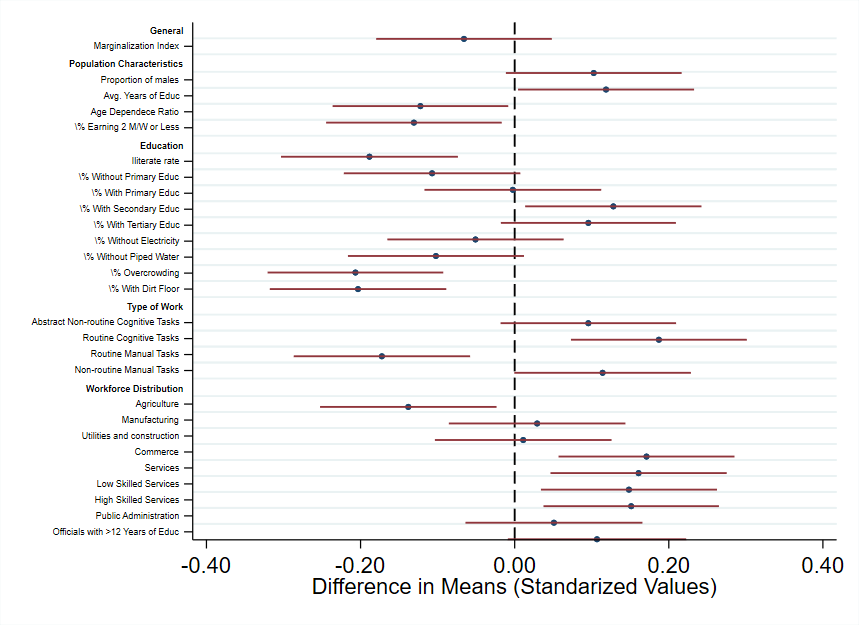
\includegraphics[width=\linewidth]{figures/obs_res_ols_sc_tr.png}
			\caption*{\footnotesize A. Observational vs OLS weights} 
		\end{subfigure} 
	\vspace{0.1cm} %\hfill
		\begin{subfigure}[t]{0.77\textwidth} 
			\centering
			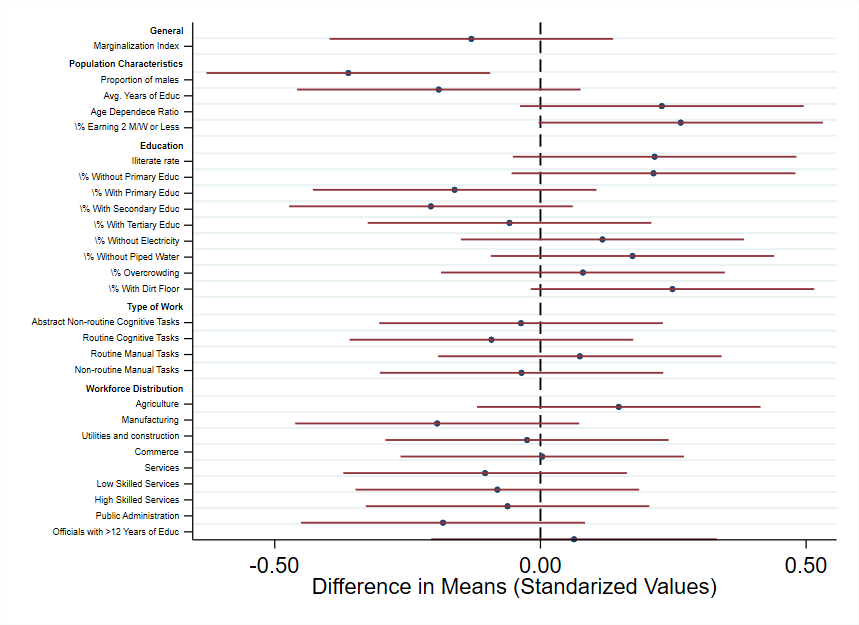
\includegraphics[width=\linewidth]{figures/obs_res_cf_sc_tr.png}
			\caption*{\footnotesize B. Observational vs IV weights} 
		\end{subfigure}
		\caption{Difference in Means of Baseline Characteristics: Observational vs Effective sample}\label{fig:late}
	
		\parbox{\textwidth}{\small 
			\vspace{2eX}
			\footnotesize	
			\sammi
		}
\end{figure}



\begin{table}[H]
	\centering
	\small
	\caption{Descriptive Statistics of Main Sample}
	\label{poly_inf}
	\resizebox{\textwidth}{!}{
		{
\def\sym#1{\ifmmode^{#1}\else\(^{#1}\)\fi}
\begin{tabular}{l*{3}{cccc}}
\hline\hline
                    &\multicolumn{2}{c}{(1)}  &\multicolumn{2}{c}{(2)}  &\multicolumn{2}{c}{(3)}           \\
                    &\multicolumn{2}{c}{Main Sample}&\multicolumn{2}{c}{Left Out}&\multicolumn{2}{c}{Means Diff}    \\
                    &        Mean&         S.D&        Mean&         S.D&        Diff         &           t\\
\hline
Marginalization Index&        0.81&        0.56&        0.90&        0.64&       -0.09\sym{*}  &     (-2.30)\\
Proportion of males &        0.48&        0.03&        0.48&        0.03&        0.00         &      (1.32)\\
Avg. Years of Educ  &        5.22&        1.60&        4.95&        1.90&        0.27\sym{*}  &      (2.34)\\
Age Dependece Ratio &        0.43&        0.05&        0.44&        0.06&       -0.01\sym{***}&     (-3.57)\\
\% Earning 2 M/W or Less&       72.51&       16.44&       76.67&       17.48&       -4.16\sym{***}&     (-3.93)\\
Iliterate rate      &       18.21&       11.64&       19.96&       14.31&       -1.75\sym{*}  &     (-2.05)\\
\% Without Primary Educ&       46.17&       15.02&       48.09&       17.62&       -1.92         &     (-1.81)\\
\% With Primary Educ&        0.24&        0.06&        0.25&        0.09&       -0.02\sym{**} &     (-3.13)\\
\% With Secondary Educ&        0.19&        0.10&        0.16&        0.11&        0.03\sym{***}&      (3.97)\\
\% With Tertiary Educ&        0.05&        0.05&        0.04&        0.07&        0.01\sym{*}  &      (1.97)\\
\% Without Electricity&        9.78&       12.05&       11.69&       15.47&       -1.91\sym{*}  &     (-2.07)\\
\% Without Piped Water&       18.88&       20.22&       18.89&       22.43&       -0.01         &     (-0.01)\\
\% Overcrowding     &       56.41&       13.63&       54.57&       15.74&        1.83         &      (1.94)\\
\% With Dirt Floor  &       30.80&       24.84&       36.35&       27.91&       -5.54\sym{**} &     (-3.29)\\
Abstract Non-routine Cognitive Tasks&        0.07&        0.05&        0.06&        0.06&        0.01         &      (1.51)\\
Routine Cognitive Tasks&        0.15&        0.09&        0.12&        0.10&        0.03\sym{***}&      (4.87)\\
Routine Manual Tasks&        0.66&        0.16&        0.71&        0.18&       -0.05\sym{***}&     (-4.37)\\
Non-routine Manual Tasks&        0.13&        0.06&        0.11&        0.06&        0.01\sym{***}&      (3.78)\\
Agriculture         &        0.44&        0.24&        0.52&        0.25&       -0.08\sym{***}&     (-4.95)\\
Manufacturing       &        0.14&        0.11&        0.12&        0.11&        0.02\sym{**} &      (2.86)\\
Utilities and construction&        0.09&        0.06&        0.09&        0.07&        0.00         &      (0.02)\\
Commerce            &        0.10&        0.06&        0.08&        0.06&        0.03\sym{***}&      (6.67)\\
Services            &        0.23&        0.12&        0.19&        0.14&        0.03\sym{***}&      (3.63)\\
Low Skilled Services&        0.10&        0.05&        0.08&        0.06&        0.02\sym{***}&      (4.48)\\
High Skilled Services&        0.10&        0.06&        0.08&        0.08&        0.02\sym{***}&      (3.57)\\
Public Administration&        0.03&        0.02&        0.03&        0.03&       -0.00         &     (-1.58)\\
Officials with >12 Years of Educ&        0.14&        0.14&        0.10&        0.15&        0.03\sym{***}&      (3.72)\\
\hline
Observations        &        2135&            &         307&            &        2442         &            \\
\hline\hline
\end{tabular}
}

	}		
	\parbox{\textwidth}{\small 
		\vspace{2eX}
		\footnotesize	
		\maintable
		\polynomial 
	}
	
	
\end{table}


%%%%%%%%%%%%%%%%%%%%%%%%%%%%%%%%%%%%%%%%%%%%%%%%%%%%%%%%%%%
\subsection{MHT}\label{ap:E}
%%%%%%%%%%%%%%%%%%%%%%%%%%%%%%%%%%%%%%%%%%%%%%%%%%%%%%%%%%%

\begin{table}[H]
	\centering
	\small
	\caption{FWER p-values: Impact of FAIS on All Outcomes by Family Type}
	\label{ap:E.1}
	
	\resizebox{!}{!}{
		
		
		

\begin{tabular}{lcccc}

\toprule

\multicolumn{1}{l}{} & \multicolumn{2}{c}{\textit{Estimates}} & \multicolumn{2}{c}{\textit{FWER p-values}} \\
\multicolumn{1}{l}{} & \multicolumn{1}{c}{\textit{Coef.}} & \multicolumn{1}{c}{\textit{S.E}} & \multicolumn{1}{c}{\textit{Anderson}} & \multicolumn{1}{c}{\textit{Wyoung}} \\ 
 
\cmidrule(l{1mm}r{1mm}){2-3} \cmidrule(l{1mm}r{1mm}){4-5}  \\

\midrule

\multicolumn{5}{c}{\textit{Panel  A: Social Infrastructure}}   \\  

\textit{Access to electric lighting}  &  0.927***  
					   & (0.344) 
					   & [0.013]  
					   & \{0.004\} \\[0.2cm]
					   
\textit{Connection to sewerage}  &  6.041***  
					   & (0.950) 
					   & [0.000]  
					   & \{0.001\} \\[0.2cm]
					   
\textit{Access piped water}  &  4.921***  
					   & (0.933) 
					   & [0.000]  
					   & \{0.001\} \\[0.2cm]
					   
\textit{Housing (floor quality)}  &  4.478***  
					   & (0.736) 
					   & [0.000]  
					   & [0.001\} \\[0.2cm]
					   
\textit{Access to sanitation}  &  -0.257  
					   & (0.572) 
					   & [0.656]  
					   & \{0.151\} \\[0.2cm]

\midrule

\multicolumn{5}{c}{\textit{Panel  B: Poverty and Mean Income}}   \\[0.2cm]  

\textit{Mean household income (log)}  &  0.026  
					   & (0.019) 
					   &  [0.303]  
					   & \{0.945\} \\[0.2cm]
					   
\textit{Food poverty rate}  &  -0.548  
					   & (0.851) 
					   &  [0.531]  
					   & \{0.945\} \\[0.2cm]
					   
\textit{Capabilities poverty rate}  &  -0.774  
					   & (0.853) 
					   &  [0.426]  
					   & \{0.945\} \\[0.2cm]
					   
\textit{Assets poverty rate}  &  -0.806  
					   & (0.770) 
					   &  [0.426]  
					   & \{0.945\} \\[0.2cm]

\midrule                                                                                      
\multicolumn{5}{c}{\textit{Panel  C: Inequality}}   \\[0.2cm]  

\textit{Gini index}  &  1.837***  
					   & (0.436) 
					   & [0.000]  
					   & \{0.001\} \\[0.2cm]
					   
\textit{Income Ratio 90/10}  &  0.239  
					   & (0.151) 
					   & [0.138]  
					   & \{0.060\} \\[0.2cm]
					   
\textit{Income Ratio 50/10}  &  0.029  
					   & (0.028) 
					   & [0.287]  
					   & \{0.136\} \\[0.2cm]
					   
\textit{Income Ratio 90/50}  &  0.110***  
					   & (0.030) 
					   & [0.001]  
					   & \{0.001\} \\[0.2cm]
					   
%\textit{$$name5_p3$$}  &  $$c1_p3_v5_starbeta$$  
%					   & ($$c1_p3_v5_se$$) 
%					   & [$$c1_p3_v5_wy$$]  
%					   & \{$$c1_p3_v5_anderson$$\} \\[0.2cm]

\midrule

\textit{Observations} 	  &   6123	\\[0.2cm]
\textit{Municipalities}   &   2119   \\[0.2cm]

\bottomrule

\end{tabular}%


		
	}		
	\parbox{\textwidth}{\small 
		\vspace{2eX}
		\footnotesize	
		\mhtnote 
	}
	
\end{table}


\begin{table}[H]
	\centering
	\small
	\caption{Indeces: Impact of FAIS on ICW Index by Family type}
	\label{ap:E.2}
	
	\resizebox{11cm}{!}{
		
		
		\begin{tabular}{lccccc}

\toprule



%\multicolumn{1}{l}{} & \multicolumn{1}{c}{\substack{\text{\it Observed} \\ \text{\it FAIS transfers} }}
%					 & \multicolumn{1}{c}{\substack{\text{\it Law-implied} \\ \text{\it FAIS transfers}}}
%					 & \multicolumn{3}{c}{\substack{\text{\it Observed} \\ \text{\it FAIS transfers} }} 
%					  \\ 

%This p option in multicolumn help with miktex but do the same as substack that works on overleaf. Worse to make aligments of title so we end up doing manually 
%\multicolumn{1}{l}{} & \multicolumn{1}{p{2cm}}{\centering{\scriptsize{ Observed \\ FAIS transfers}}}
%					 & \multicolumn{1}{p{2cm}}{\centering{\scriptsize{ Law-implied \\  FAIS transfers}}}
%					 & \multicolumn{3}{p{2cm}}{\centering{\scriptsize{ Observed FAIS \\  transfers}}}
%					 \\ 
\multicolumn{1}{l}{} & \multicolumn{1}{c}{\scriptsize{ Observed   }}
					 & \multicolumn{1}{c}{\scriptsize{ Law-implied }}
					 & \multicolumn{3}{c}{\scriptsize{ Observed   }}
					 \\ 
\multicolumn{1}{l}{} & \multicolumn{1}{c}{\scriptsize{ FAIS  }}
					 & \multicolumn{1}{c}{\scriptsize{ FAIS  }}
					 & \multicolumn{3}{c}{\scriptsize{ FAIS  }}
					 \\ 
					 
\multicolumn{1}{l}{} & \multicolumn{1}{c}{\footnotesize{(OLS)}}
					 & \multicolumn{1}{c}{\footnotesize{(RF)}}
					 & \multicolumn{3}{c}{\footnotesize{(2SLS)}} 
					  \\ 





\cmidrule(lr{1mm}){2-2} 
\cmidrule(lr{1mm}){3-3} 
\cmidrule(lr{1mm}){4-6}  % \\ was before, it was creating an extra additional line


\multicolumn{1}{l}{} &  \multicolumn{1}{c}{(1)} &
						\multicolumn{1}{c}{(2)} & 
						\multicolumn{1}{c}{(3)} & 
						\multicolumn{1}{c}{(4)} & 
						\multicolumn{1}{c}{(5)} \\

\midrule
                                            

% 1st row 
\textit{Social infrastructure index}   &  0.042***   &
						   0.071***   &
						   0.102***   &  
   						   0.077***   &  
						   0.086***   \\  
						   

\vspace{4pt} &  \footnotesize{(0.009)}  &
			    \footnotesize{(0.019)}  &
			    \footnotesize{(0.020)}  &
				\footnotesize{(0.019)}  &
				\footnotesize{(0.023)}  \\

\vspace{4pt} &  \footnotesize{[--]}  &
			    \footnotesize{[--]}  &
			    \footnotesize{[844]}  &
				\footnotesize{[841]}  &
				\footnotesize{[605]}  \\

% 2nd row 
\textit{Poverty and mean income index}   &  -0.017   &
						   0.030   &
						   -0.001   &  
   						   0.021   &  
						   0.038   \\  
						   

\vspace{4pt} &  \footnotesize{(0.023)}   &
			    \footnotesize{(0.045)}   &
			    \footnotesize{(0.046)}   &
				\footnotesize{(0.046)}   &
				\footnotesize{(0.056)}   \\

\vspace{4pt} &  \footnotesize{[--]}   &
			    \footnotesize{[--]}   &
			    \footnotesize{[844]}   &
				\footnotesize{[845]}   &
				\footnotesize{[591]}   \\

% 3rd row  			
\textit{Inequality index}   &  0.201***   &
						   0.175**   &
						   0.193***   &  
   						   0.196***   &  
						   0.216**   \\  
						   
\vspace{4pt} &  \footnotesize{(0.037)}   &
			    \footnotesize{(0.071)}   &
			    \footnotesize{(0.072)}   &
				\footnotesize{(0.073)}   &
				\footnotesize{(0.088)}   \\

\vspace{4pt} &  \footnotesize{[--]}   &
			    \footnotesize{[--]}   &
			    \footnotesize{[844]}   &
				\footnotesize{[836]}   &
				\footnotesize{[588]}   \\


\midrule
{\bf Controls}    					&	   &   
										   & 
										   & 
										   &
										   \\


\textit{Municipality and year FE}    &	$\checkmark$   &   
										$\checkmark$   & 
										$\checkmark$   & 
										$\checkmark$   &
										$\checkmark$   \\

\textit{Formula inputs}  	& 	$\checkmark$    &   
								$\checkmark$    & 
								$\checkmark$    & 
								$\checkmark$    &
								$\checkmark$    \\

\textit{Dep. var pre-trends}  & 			    &   
												& 
												& 
								$\checkmark$    &
								$\checkmark$    \\

\textit{Fiscal revenues}  	& 					&   
												& 
												& 
												&
								$\checkmark$   \\


\midrule		


Observations 			&	 6143   &   
							 6143   & 
							 6123   & 
							 6123   &
							 6107   \\

Municipalities  		&    2154   &   
							 2154   & 
							 2119   & 
							 2119   &
							 2118   \\


\bottomrule

\end{tabular}%

		
	}		
	\parbox{\textwidth}{\small 
		\vspace{2eX}
		\footnotesize	
		\indicestables
	}
	
\end{table}



%%%%%%%%%%%%%%%%%%%%%%%%%%%%%%%%%%%%%%%%%%%%%%%%%%%%%%%%%%%
%\subsubsubsection{Migration}
%%%%%%%%%%%%%%%%%%%%%%%%%%%%%%%%%%%%%%%%%%%%%%%%%%%%%%%%%%%

%\begin{table}[H]
%	\centering
%	\small
%	\caption{The Impact of FAIS on Migration}
%	\label{mig}
%	\resizebox{11cm}{!}{
%		\begin{tabular}{lccccc}

\toprule



%\multicolumn{1}{l}{} & \multicolumn{1}{c}{\substack{\text{\it Observed} \\ \text{\it FAIS transfers} }}
%					 & \multicolumn{1}{c}{\substack{\text{\it Law-implied} \\ \text{\it FAIS transfers}}}
%					 & \multicolumn{3}{c}{\substack{\text{\it Observed} \\ \text{\it FAIS transfers} }} 
%					  \\ 

%This p option in multicolumn help with miktex but do the same as substack that works on overleaf. Worse to make aligments of title so we end up doing manually 
%\multicolumn{1}{l}{} & \multicolumn{1}{p{2cm}}{\centering{\scriptsize{ Observed \\ FAIS transfers}}}
%					 & \multicolumn{1}{p{2cm}}{\centering{\scriptsize{ Law-implied \\  FAIS transfers}}}
%					 & \multicolumn{3}{p{2cm}}{\centering{\scriptsize{ Observed FAIS \\  transfers}}}
%					 \\ 
\multicolumn{1}{l}{} & \multicolumn{1}{c}{\scriptsize{ Observed   }}
					 & \multicolumn{1}{c}{\scriptsize{ Law-implied }}
					 & \multicolumn{3}{c}{\scriptsize{ Observed   }}
					 \\ 
\multicolumn{1}{l}{} & \multicolumn{1}{c}{\scriptsize{ FAIS  }}
					 & \multicolumn{1}{c}{\scriptsize{ FAIS  }}
					 & \multicolumn{3}{c}{\scriptsize{ FAIS  }}
					 \\ 
					 
\multicolumn{1}{l}{} & \multicolumn{1}{c}{\footnotesize{(OLS)}}
					 & \multicolumn{1}{c}{\footnotesize{(RF)}}
					 & \multicolumn{3}{c}{\footnotesize{(2SLS)}} 
					  \\ 





\cmidrule(lr{1mm}){2-2} 
\cmidrule(lr{1mm}){3-3} 
\cmidrule(lr{1mm}){4-6}  % \\ was before, it was creating an extra additional line


\multicolumn{1}{l}{} &  \multicolumn{1}{c}{(1)} &
						\multicolumn{1}{c}{(2)} & 
						\multicolumn{1}{c}{(3)} & 
						\multicolumn{1}{c}{(4)} & 
						\multicolumn{1}{c}{(5)}  \\ 


\midrule

%\multicolumn{7}{c}{\textit{Panel   A: Direct policy outcomes on infrastructure}} \\                                                          

% 1st row 
\textit{Total Population}   &  -0.009   &
						   -0.158***   &
						   -0.213***   &  
   						   -0.169***   &  
						   -0.193***   \\  
						   

\vspace{4pt} &  \footnotesize{(0.006)}  &
			    \footnotesize{(0.024)}  &
			    \footnotesize{(0.027)}  &
				\footnotesize{(0.026)}  &
				\footnotesize{(0.032)}  \\

\vspace{4pt} &  \footnotesize{[--]}  &
			    \footnotesize{[--]}  &
			    \footnotesize{[844]}  &
				\footnotesize{[809]}  &
				\footnotesize{[590]}  \\

% 2nd row 
\textit{Adult population}   &  -0.008**   &
						   -0.084***   &
						   -0.147***   &  
   						   -0.090***   &  
						   -0.104***   \\  
						   

\vspace{4pt} &  \footnotesize{(0.004)}   &
			    \footnotesize{(0.014)}   &
			    \footnotesize{(0.017)}   &
				\footnotesize{(0.015)}   &
				\footnotesize{(0.018)}   \\

\vspace{4pt} &  \footnotesize{[--]}   &
			    \footnotesize{[--]}   &
			    \footnotesize{[844]}   &
				\footnotesize{[688]}   &
				\footnotesize{[559]}   \\

% 3rd row  			
\textit{Primary or less}   &  -0.003   &
						   -0.054***   &
						   -0.102***   &  
   						   -0.057***   &  
						   -0.066***   \\  
						   
\vspace{4pt} &  \footnotesize{(0.004)}   &
			    \footnotesize{(0.014)}   &
			    \footnotesize{(0.014)}   &
				\footnotesize{(0.014)}   &
				\footnotesize{(0.017)}   \\

\vspace{4pt} &  \footnotesize{[--]}   &
			    \footnotesize{[--]}   &
			    \footnotesize{[844]}   &
				\footnotesize{[786]}   &
				\footnotesize{[605]}   \\

% 4th row  				
\textit{Secondary education}   &  -0.004   &
						   -0.085***   &
						   -0.108***   &  
   						   -0.093***   &  
						   -0.104***   \\  
						   

\vspace{4pt} &  \footnotesize{(0.006)}   &
			    \footnotesize{(0.019)}   &
			    \footnotesize{(0.021)}   &
				\footnotesize{(0.021)}   &
				\footnotesize{(0.024)}   \\

\vspace{4pt} &  \footnotesize{[--]}   &
			    \footnotesize{[--]}   &
			    \footnotesize{[844]}   &
				\footnotesize{[816]}   &
				\footnotesize{[615]}   \\

% 5th row  				
\textit{College}   &  0.062***   &
						   0.071**   &
						   0.069*   &  
   						   0.066*   &  
						   0.088**   \\  
						   

\vspace{4pt} &  \footnotesize{(0.013)}   &
			    \footnotesize{(0.034)}   &
			    \footnotesize{(0.037)}   &
				\footnotesize{(0.036)}   &
				\footnotesize{(0.043)}   \\

\vspace{4pt} &  \footnotesize{[--]}   &
			    \footnotesize{[--]}   &
			    \footnotesize{[838]}   &
				\footnotesize{[822]}   &
				\footnotesize{[584]}   \\

% 6th row  				
\textit{Young (15-25)}   &  -0.017***   &
						   -0.113***   &
						   -0.172***   &  
   						   -0.118***   &  
						   -0.137***   \\  
						   

\vspace{4pt} &  \footnotesize{(0.005)}   &
			    \footnotesize{(0.016)}   &
			    \footnotesize{(0.019)}   &
				\footnotesize{(0.017)}   &
				\footnotesize{(0.020)}   \\

\vspace{4pt} &  \footnotesize{[--]}   &
			    \footnotesize{[--]}   &
			    \footnotesize{[844]}   &
				\footnotesize{[774]}   &
				\footnotesize{[606]}   \\


% 7th row  				
\textit{Prime age (15-55)}   &  -0.007*   &
						   -0.083***   &
						   -0.148***   &  
   						   -0.089***   &  
						   -0.102***   \\  
						   

\vspace{4pt} &  \footnotesize{(0.004)}   &
			    \footnotesize{(0.015)}   &
			    \footnotesize{(0.019)}   &
				\footnotesize{(0.017)}   &
				\footnotesize{(0.020)}   \\

\vspace{4pt} &  \footnotesize{[--]}   &
			    \footnotesize{[--]}   &
			    \footnotesize{[844]}   &
				\footnotesize{[745]}   &
				\footnotesize{[594]}   \\

% 8th row  				
\textit{Old (+55)}   &  -0.006   &
						   -0.079***   &
						   -0.129***   &  
   						   -0.082***   &  
						   -0.098***   \\  
						   

\vspace{4pt} &  \footnotesize{(0.004)}   &
			    \footnotesize{(0.011)}   &
			    \footnotesize{(0.013)}   &
				\footnotesize{(0.012)}   &
				\footnotesize{(0.014)}   \\

\vspace{4pt} &  \footnotesize{[--]}   &
			    \footnotesize{[--]}   &
			    \footnotesize{[844]}   &
				\footnotesize{[802]}   &
				\footnotesize{[583]}   \\


\midrule
{\bf Controls}    					&	   &   
										   & 
										   & 
										   &
										   \\


\textit{Municipality and year FE}    &	$\checkmark$   &   
										$\checkmark$   & 
										$\checkmark$   & 
										$\checkmark$   &
										$\checkmark$   \\

\textit{Formula inputs}  	& 	$\checkmark$    &   
								$\checkmark$    & 
								$\checkmark$    & 
								$\checkmark$    &
								$\checkmark$    \\

\textit{Dep. var pre-trends}  & 			    &   
												& 
												& 
								$\checkmark$    &
								$\checkmark$    \\

\textit{Fiscal revenues}  	& 					&   
												& 
												& 
												&
								$\checkmark$   \\


\midrule		


Observations 			&	 6143   &   
							 6143   & 
							 6123   & 
							 6123   &
							 6107   \\

Municipalities  		&   2154   &   
							 2154   & 
							 2119   & 
							 2119   &
							 2118   \\


\bottomrule

\end{tabular}%

%	}		
%	\parbox{\textwidth}{\small 
%		\vspace{2eX}
%		\footnotesize	
%		\maintable
%		\polynomial 
%	}
%\end{table}




%\subsubsubsection{Estimates by deciles (upon request)}
%\begin{table}[H]
%	\centering
%	\small
%	\caption{Heterogeneity: Impact of FAIS on the Income Distribution Percentiles by Urban/Rural}
%	\label{ineq_urb}
%	\resizebox{0.6\textwidth}{!}{
%		\begin{tabular}{lccc}

\toprule



\multicolumn{1}{l}{} & \multicolumn{3}{c}{\footnotesize{Observed FAIS Transfers (2SLS)}} \\ 


\cmidrule(lr{1mm}){2-2} 
\cmidrule(lr{1mm}){3-3} 
\cmidrule(lr{1mm}){4-4}  % "\\" was before, it was creating an extra additional line


\multicolumn{1}{l}{} &  \multicolumn{1}{c}{All} &
						\multicolumn{1}{c}{Urban} & 
						\multicolumn{1}{c}{Rural} \\
\multicolumn{1}{l}{} &  \multicolumn{1}{c}{(1)} &
						\multicolumn{1}{c}{(2)} & 
						\multicolumn{1}{c}{(3)} \\
						

\midrule

%\multicolumn{7}{c}{\textit{Panel   A: Direct policy outcomes on infrastructure}} \\                                                          

% 1st row 
\textit{10 pctle}   &  -0.023   
						&  0.033  
						&  -0.083***   \\

\vspace{4pt} &  \footnotesize{(0.020)}   & 
			    \footnotesize{(0.027)}   & 
			    \footnotesize{(0.031)}    \\          


\vspace{4pt} &  \footnotesize{[847]}   & 
			    \footnotesize{[404]}   & 
			    \footnotesize{[347]}    \\          




% 2nd row 
\textit{20 pctle}   	&  -0.020   
							&  0.015  
							&  -0.070**   \\

\vspace{4pt} &  \footnotesize{(0.019)}   & 
			    \footnotesize{(0.024)}   & 
			    \footnotesize{(0.029)}   \\          


\vspace{4pt} &  \footnotesize{[848]}   & 
			    \footnotesize{[403]}   & 
			    \footnotesize{[346]}   \\          


% 3rd row  			
\textit{30 pctle}   	&  -0.013   
							&  0.009  
							&  -0.059**   \\

\vspace{4pt} &  \footnotesize{(0.018)}   & 
			    \footnotesize{(0.022)}   & 
			    \footnotesize{(0.029)}   \\          


\vspace{4pt} &  \footnotesize{[847]}   & 
			    \footnotesize{[402]}   & 
			    \footnotesize{[346]}   \\          



% 4th row  				
\textit{40 pctle}   	&  -0.006   
							&  0.009  
							&  -0.051*   \\

\vspace{4pt} &  \footnotesize{(0.018)}   & 
			    \footnotesize{(0.022)}   & 
			    \footnotesize{(0.029)}   \\          


\vspace{4pt} &  \footnotesize{[845]}   & 
			    \footnotesize{[402]}   & 
			    \footnotesize{[345]}   \\          



% 5th row 
\textit{50 pctle}   	&  0.003   
							&  0.010  
							&  -0.041   \\

\vspace{4pt} &  \footnotesize{(0.018)}   & 
			    \footnotesize{(0.022)}   & 
			    \footnotesize{(0.029)}   \\          


\vspace{4pt} &  \footnotesize{[842]}   & 
			    \footnotesize{[401]}   & 
			    \footnotesize{[343]}   \\          


% 6th row 
\textit{60 pctle}   	&  0.012   
							&  0.014  
							&  -0.031   \\

\vspace{4pt} &  \footnotesize{(0.018)}   & 
			    \footnotesize{(0.022)}   & 
			    \footnotesize{(0.030)}   \\          


\vspace{4pt} &  \footnotesize{[840]}   & 
			    \footnotesize{[400]}   & 
			    \footnotesize{[342]}   \\          

% 7th row 
\textit{70 pctle}   	&  0.023   
							&  0.019  
							&  -0.020   \\

\vspace{4pt} &  \footnotesize{(0.019)}   & 
			    \footnotesize{(0.023)}   & 
			    \footnotesize{(0.031)}   \\          


\vspace{4pt} &  \footnotesize{[837]}   & 
			    \footnotesize{[400]}   & 
			    \footnotesize{[341]}   \\          

% 8th row 
\textit{80 pctle}   	&  0.036*   
							&  0.028  
							&  -0.006   \\

\vspace{4pt} &  \footnotesize{(0.020)}   & 
			    \footnotesize{(0.024)}   & 
			    \footnotesize{(0.033)}   \\          


\vspace{4pt} &  \footnotesize{[835]}   & 
			    \footnotesize{[399]}   & 
			    \footnotesize{[340]}   \\          

% 9th row 
\textit{90 pctle}   	&  0.055**   
							&  0.040  
							&  0.015   \\

\vspace{4pt} &  \footnotesize{(0.022)}   & 
			    \footnotesize{(0.027)}   & 
			    \footnotesize{(0.036)}   \\          


\vspace{4pt} &  \footnotesize{[833]}   & 
			    \footnotesize{[399]}   & 
			    \footnotesize{[339]}   \\          



\midrule
{\bf Controls}    					&	   &   
										   & 
										   \\


\textit{Municipality and year FE}    &	$\checkmark$   & 
										$\checkmark$   & 
										$\checkmark$   \\

\textit{Dep. var pre-trends}  & $\checkmark$   &   
								$\checkmark$   & 
								$\checkmark$   \\
								
								
								
\midrule		

Observations 			&	 6123   &  
							 2949   & 
							 3063   \\

Municipalities  		&   2119    &   
							 1020   & 
							 1089    \\
\bottomrule

\end{tabular}%

%	}		
%	\parbox{\textwidth}{\small 
%		\vspace{2eX}
%		\footnotesize	
%		\maintable
%		\urban 
%	}
%\end{table}

\end{document}